% !TeX encoding=utf8
% !TeX spellcheck = de_DE
% !TeX root = ../Diploma.tex

\chapter{Konzept des Clients}\label{sec:conceptClient}
In diesem Kapitel soll die Planung des Schachclients näher erläutert werden, welches als Grundbaustein für die Implementierung dienen soll. Dabei dient der erste Abschnitt zur Beschreibung der benötigten Anforderung, welche der Client erfüllen soll. Der zweiten Abschnitt sollen der Visualisierung und Beschreibung der einzelnen Ansichten dienen, welche für eine bequeme Nutzerinteraktion benötigt werden.

\section{Anforderungen}\label{sec:anforderungenClient}
Grundlegen soll der Client als Visualisierung des Servers dienen. Dafür soll dieser eine Verwaltung von Playern und Matches bereitstellen, inklusive der Möglichkeit zum Anlegen neuer bzw. bearbeiten schon angelegter Einträge. Um anschließend auch Schach spielen zu können muss der Client dafür eine komfortable Möglichkeit, in Form eines virtuellen Schachbrettes, bieten.\\
\\
Als Grundanforderung dafür muss der Client natürlich mit dem Server kommunizieren können. Dafür muss dieser Requests senden und die empfangenen Response-Nachrichten verarbeiten können. Da der Server für manche Request spezielle Parameter benötigt, wie zum Beispiel einen String in der \gls{SAN}, müssen diese gegebenenfalls ermittelt werden können.\\
\\
Für ein bequemes Spielerlebnis soll der Client ein gestartetes Match automatisch aktualisieren, sobald sich die Daten auf dem Server verändert haben. Um dies zu realisieren soll ein einfaches Polling-Verfahren implementiert werden.\\
\\ 
Die letzte Grundanforderung soll eine innovative und benutzerfreundliche Bedienung der Anwendung sein, so das der Nutzer keinerlei Kenntnisse, bis auf die Schachregeln, besitzen muss.

\section{Mockup-Entwicklung der benötigten Client-Ansichten}\label{sec:views}
In diesem Abschnitt sollen die im \hyperref[sec:anforderungenClient]{Kapitel~\ref{sec:anforderungenClient}} zuvor definierten Anforderungen konkretisiert und visuell aufbereitet werden. Ziel soll dabei die Erstellung von Mockups der einzelnen Ansichten sein, um die Implementierung zu vereinfachen bzw. zu beschleunigen.

\subsection{Startansicht}\label{sec:startView}
Diese Ansicht soll als Ausgangspunkt für die Nutzer dienen. Sie sollen zurückgegeben werden, sobald die Root-\gls{URL} aufgerufen wurde. Mithilfe der Startansicht soll dem Nutzer die Möglichkeit bereitgestellt werden zur Player-Ansicht bzw. zur Match-Ansicht zu wechseln. Dafür soll ihm jeweils ein Button zum Auslösen dieses Wechsels zur Verfügung gestellt werden.\\
\\
Die \hyperref[fig:startView]{Abbildung~\ref{fig:startView}} visualisiert dabei die zuvor definierten Anforderungen an die Startansicht.
\begin{figure}[htb]
	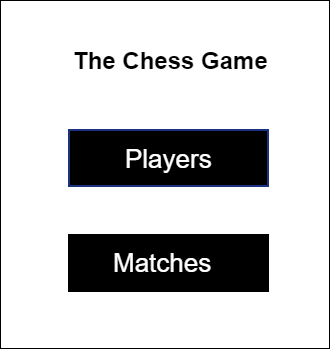
\includegraphics[width=0.9\textwidth]{images/start-view.png}
	\caption{Mockup: Startansicht des Clients}
	\label{fig:startView}
\end{figure}

\subsection{Player-Ansicht}\label{sec:playerView}
Mit dieser Ansicht soll der Nutzer die Möglichkeit erhalten alle angelegten Player zu verwalten. Dafür soll ihm eine Tabelle für die Übersicht und ein Formular zum anlegen neuer oder bearbeiten bereits angelegter Player bereitgestellt werden. Über eine Spalte innerhalb der Tabelle sollen Buttons zur Verfügung stehen, über welche ein Player bearbeitet oder gelöscht werden kann.\\
\\
Aus diesen gegebenen Anforderungen wurde das Mockup aus der \hyperref[fig:playerView]{Abbildung~\ref{fig:playerView}} entworfen, um diese visuell hervorzuheben.
\begin{figure}[htb]
	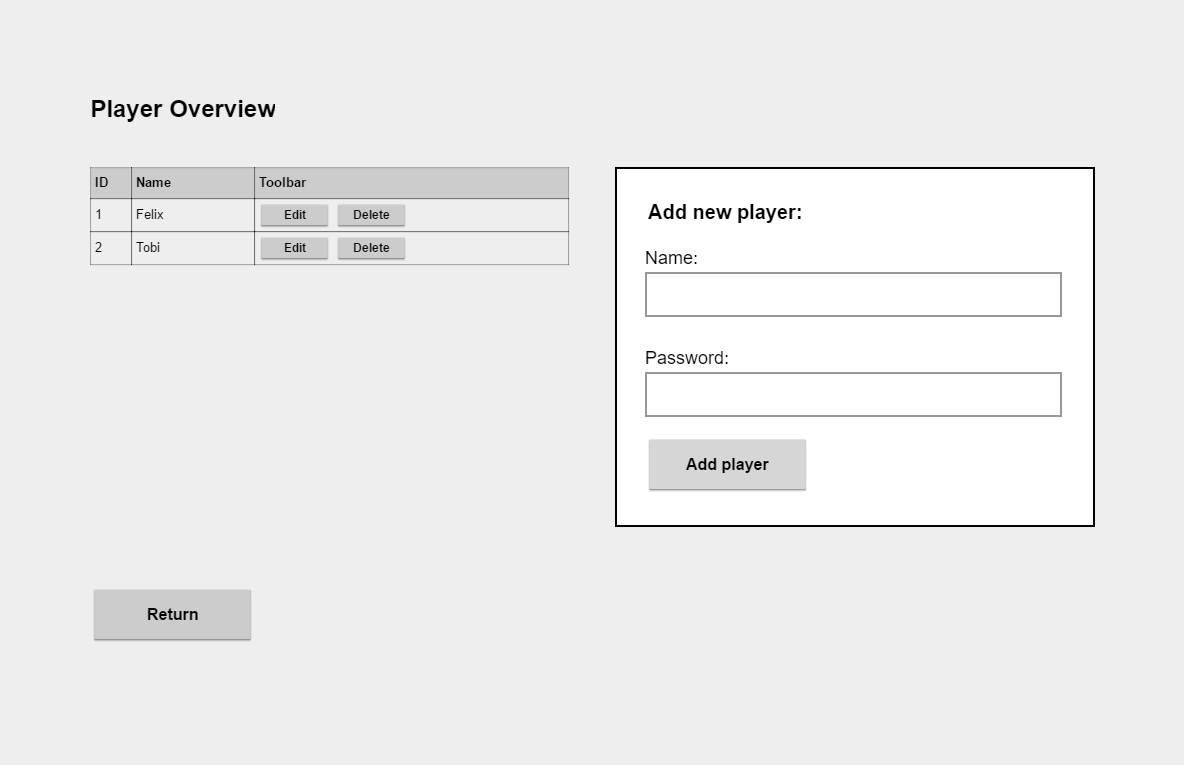
\includegraphics[width=0.9\textwidth]{images/player-view.png}
	\caption{Mockup: Player-Ansicht des Clients}
	\label{fig:playerView}
\end{figure}

\subsection{Match-Ansicht}\label{sec:matchView}
Mithilfe der Match-Ansicht soll dem Nutzer eine Ansicht zur Match-Verwaltung zur Verfügung stehen. Um dabei die Konsistenz zu wahren ist auch diese genau so aufgebaut wie die Player-Ansicht. Mit dem Unterschied das ein Match nicht gelöscht aber dafür gestartet werden kann. Daher ändern sich geringfügig die Buttons in der Tabelle.\\
\\
Dabei werden die Anforderungen durch die \hyperref[fig:matchView]{Abbildung~\ref{fig:matchView}} grafisch dargestellt.
\begin{figure}[htb]
	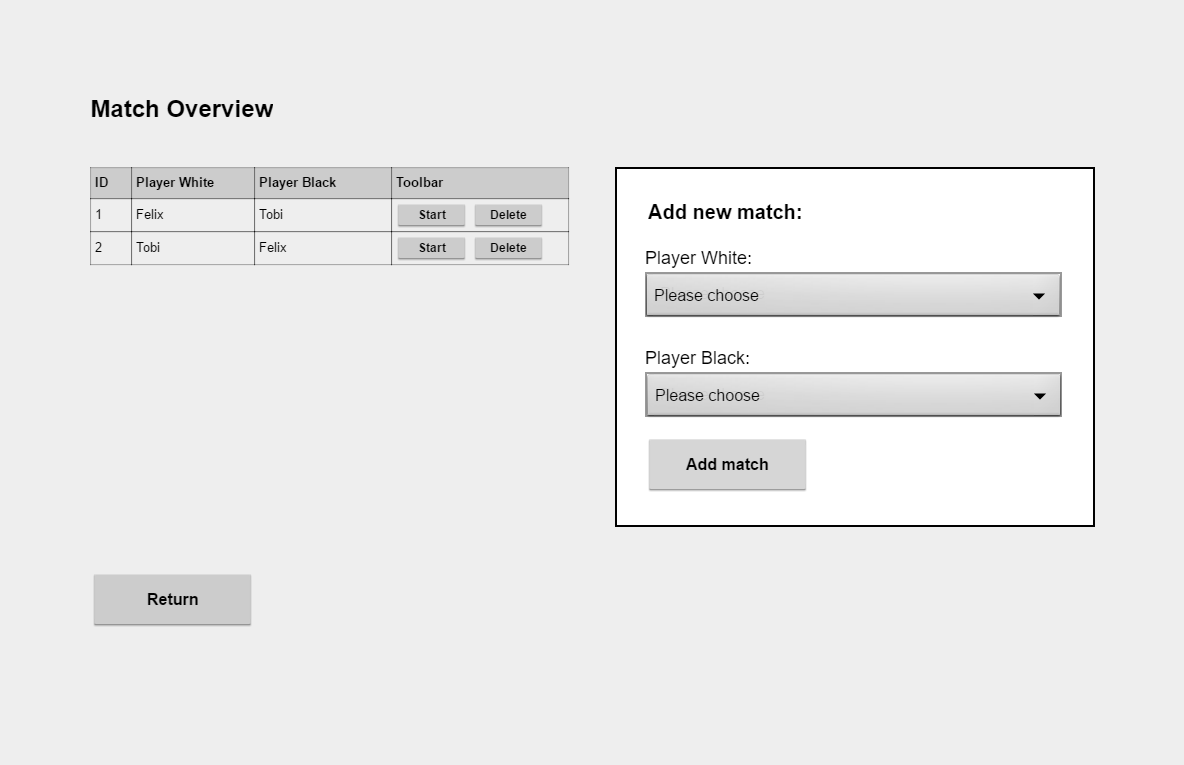
\includegraphics[width=0.9\textwidth]{images/match-view.png}
	\caption{Mockup: Match-Ansicht des Clients}
	\label{fig:matchView}
\end{figure}

\subsection{Ansicht eines gestarteten Matches}\label{sec:gameView}
Mithilfe dieser Ansicht soll dem Nutzer ermöglicht werden ein gestartetes Match zu spielen. Dafür wird in erster Linie ein Schachbrett benötigt, auf welchem die Figuren dargestellt werden. Mittels \enquote{Drag \& Drop} soll der Nutzer anschließend Spielfiguren bewegen können. Für eine einfachere Bedienung und zur Unterstützung des Verständnisses der Schachregeln, sollen alle möglichen Züge einer Figur hervorgehoben werden, sobald über diese mit der Maus gefahren wird. Da Informationen über bereits geschmissene Figuren oder welche Züge bisher getätigt wurden sehr hilfreich sein können, sollen diese neben dem Schachbrett dargestellt werden. \\
\\
Anhand dieser Kriterien an die Ansicht eines gestarteten Matches wurde das Mockup aus der \hyperref[fig:gameView]{Abbildung~\ref{fig:gameView}} entwickelt.
\begin{figure}[htb]
	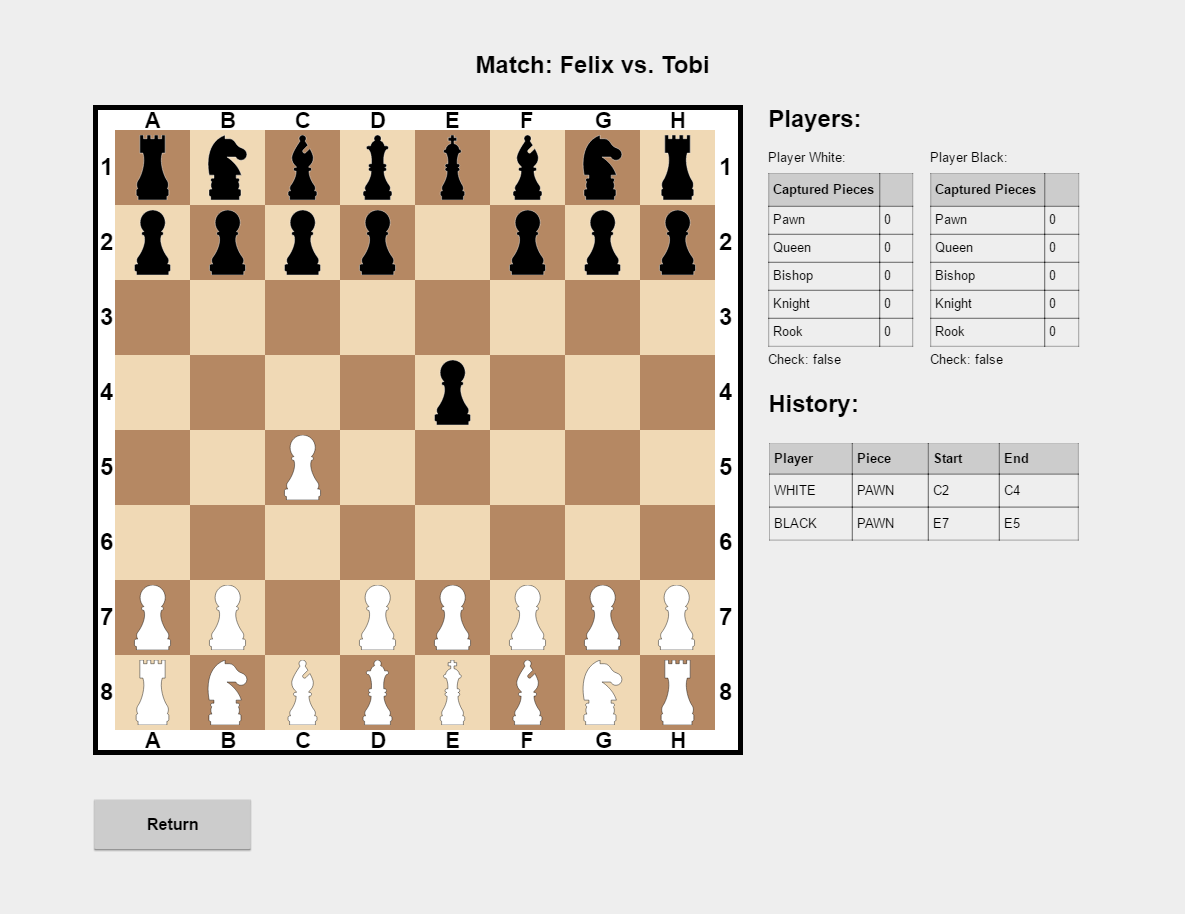
\includegraphics[width=0.9\textwidth]{images/game-view.png}
	\caption{Mockup: Ansicht eines gestarteten Matches}
	\label{fig:gameView}
\end{figure}


